% Uncomment this line for on-screen presentation
\documentclass[xcolor={dvipsnames}]{beamer}\usepackage{etoolbox}\newtoggle{printable}\togglefalse{printable}

% Uncomment this line for printable slides (disable animations and don't waste ink)
%\documentclass[handout, xcolor={dvipsnames}]{beamer}\usepackage{etoolbox}\newtoggle{printable}\toggletrue{printable}

% Adjust these for the path of the theme and its graphics, relative to this file
%\usepackage{beamerthemeFalmouthGamesAcademy}
\usepackage{../../beamerthemeFalmouthGamesAcademy}
\graphicspath{ {../../} }

% Default language for code listings
\lstset{language=C++,
		morekeywords={each,in}
}

\begin{document}
\title{Programming Practice VII}   
\subtitle{BSc Computing for Games}

\frame{\titlepage} 

\part{Morning}
\frame{\partpage}

\begin{frame}{Collaborative Project}
	In the morning session you will:
	
	\begin{itemize}
		\item \textbf{Write} the source code for the collaborative game.
		\begin{itemize}
			\item Remember to update the Trello board and check your code into the shared repository.
			\item Use pair programming where appropriate.
		\end{itemize}
	\end{itemize}
\end{frame}

\part{Afternoon}
\frame{\partpage}

\begin{frame}{Collaborative Project}
	In the afternoon session you will:
	
	\begin{itemize}
		\item \textbf{Write} the source code for the collaborative game.
		\begin{itemize}
			\item Remember to update the Trello board and check your code into the shared repository.
			\item Use pair programming where appropriate.
		\end{itemize}
		\vspace{2ex}
		\item \textbf{Write and update} the team's weekly reports.
		\item\textbf{Prepare} for the Sprint Review and Sprint Retrospective.
		\item \textbf{Complete} the team evaluation, peer evaluation, and self-evaluation forms.
	\end{itemize}
\end{frame}

% -------------------------------------------------------

%\part{The compiler}
%\frame{\partpage}
%
%\begin{frame}
%	\frametitle{The build process}
%	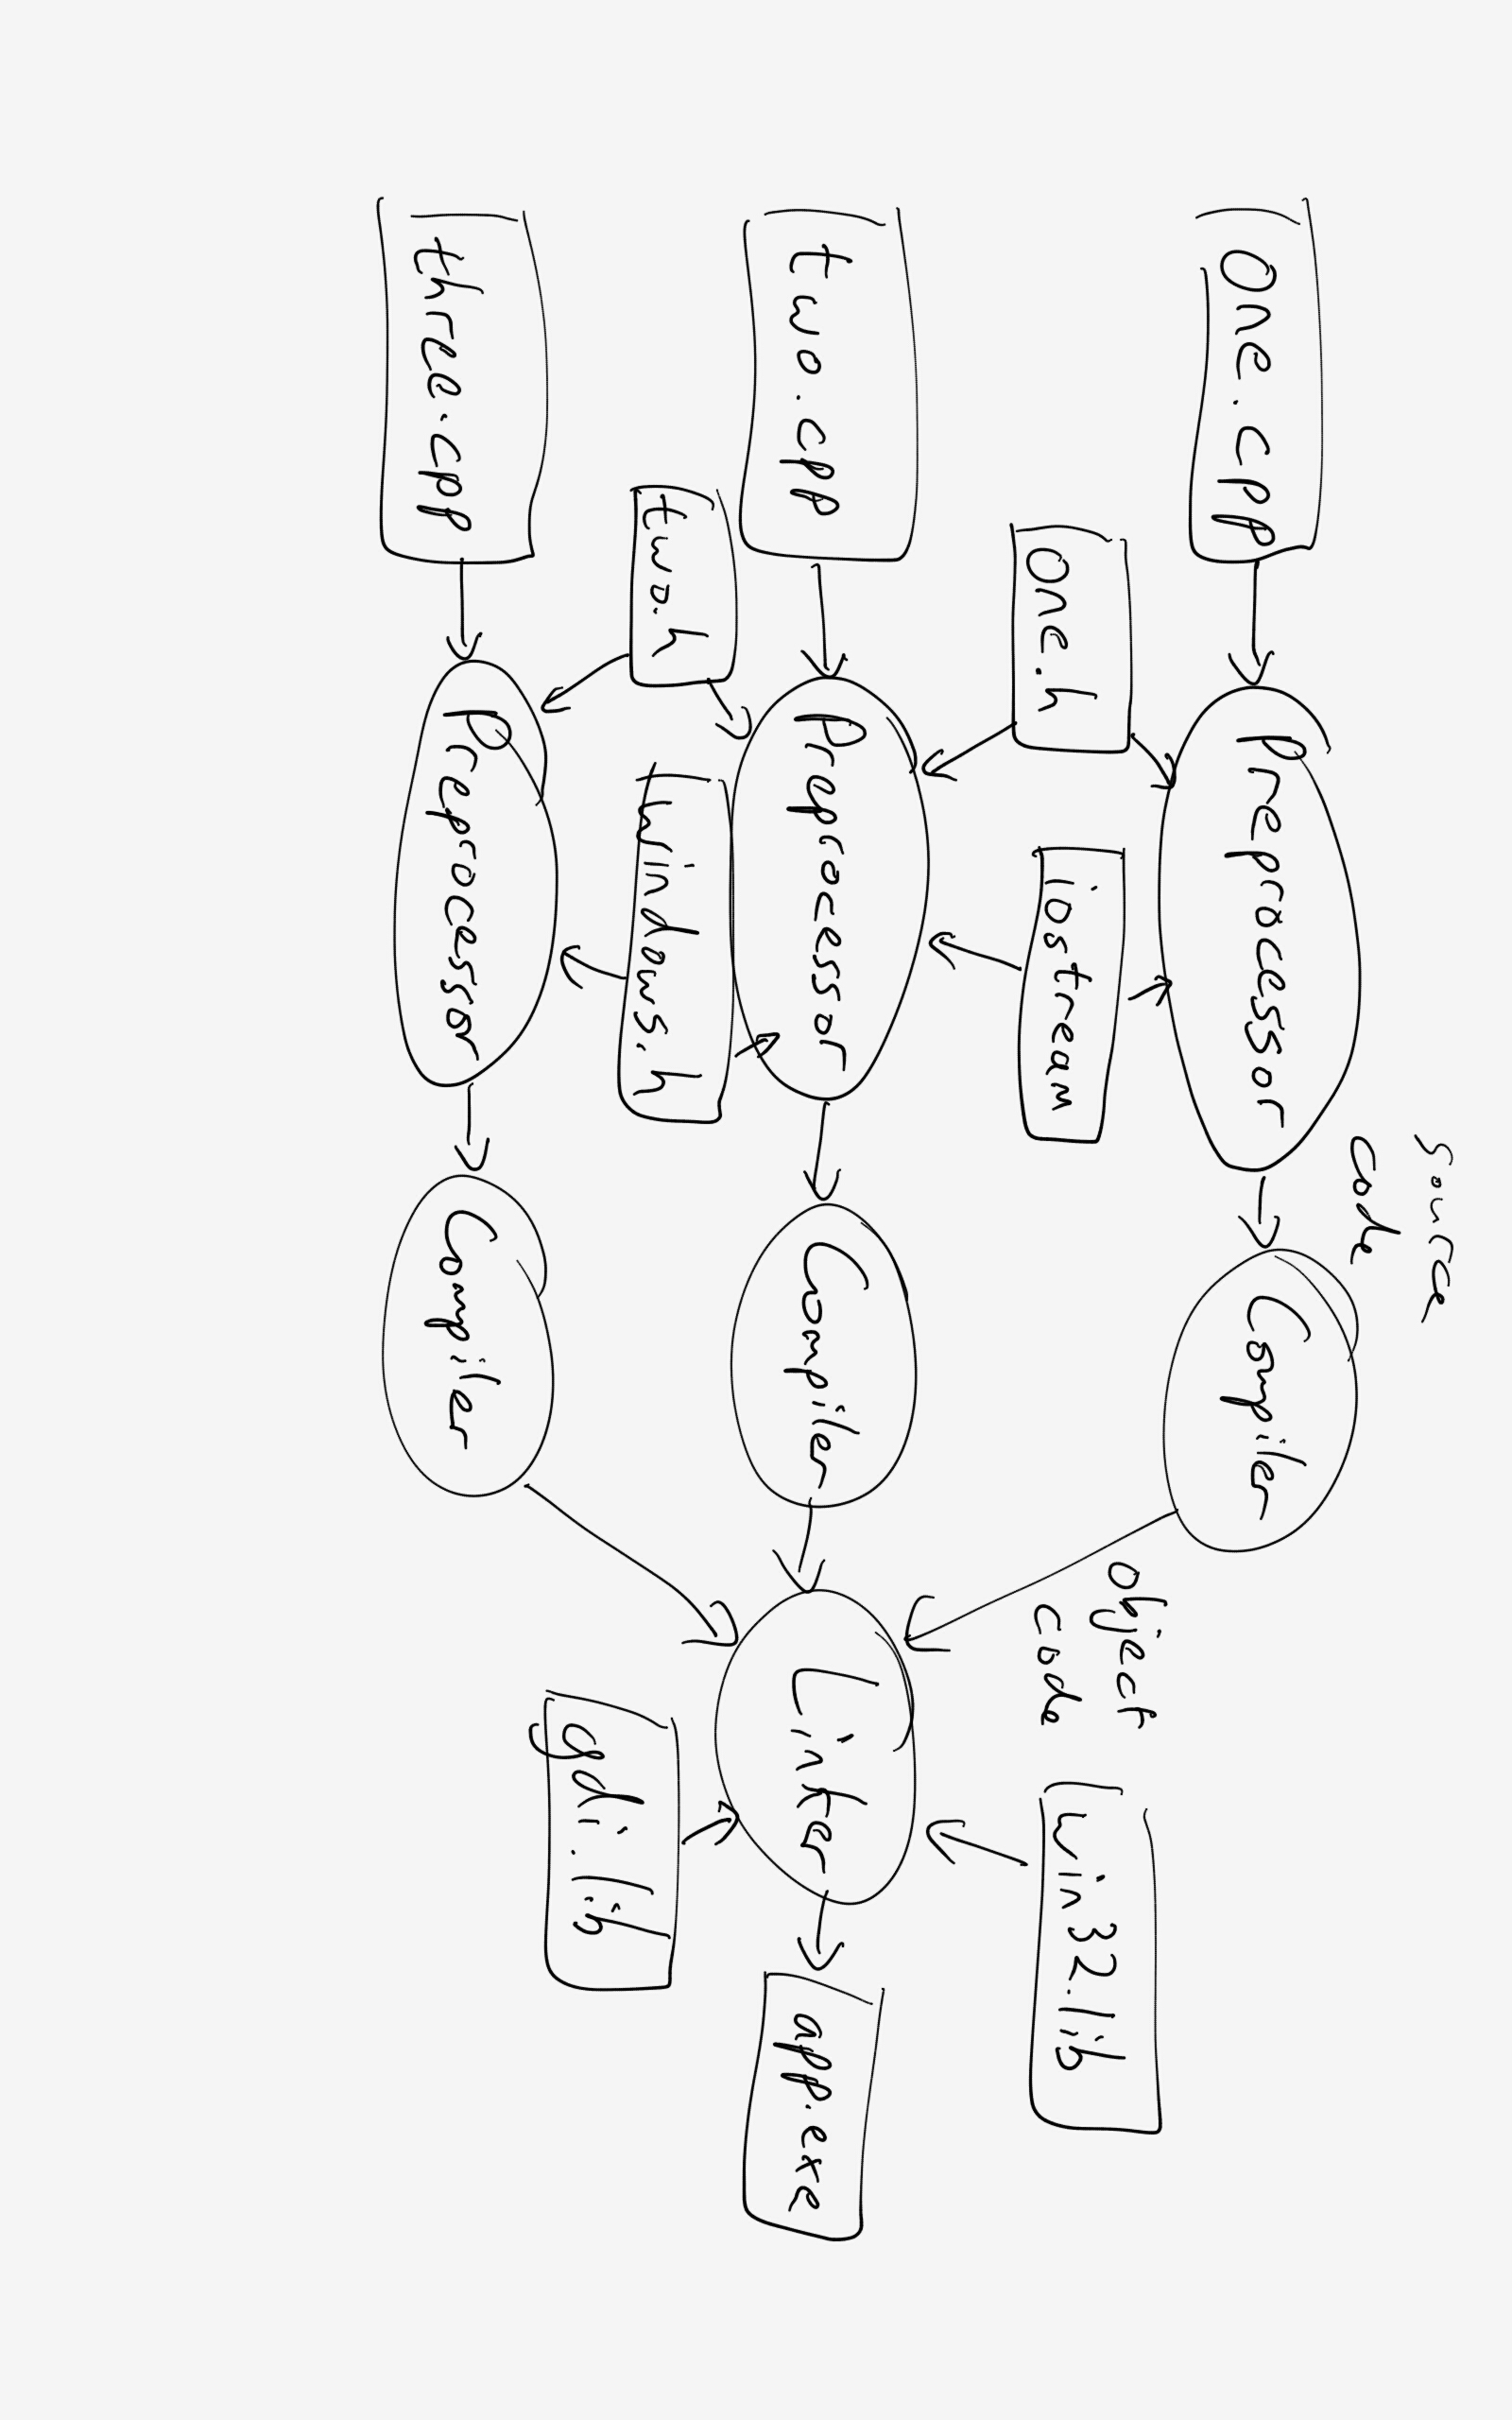
\includegraphics[height=\textwidth,angle=90]{compiler_sketch}
%\end{frame}

\end{document}
